\documentclass[a4paper]{article}

\usepackage{amsfonts, amsmath, amssymb, amsthm}
\usepackage{graphicx}
\usepackage{fullpage}
\usepackage{float}
\usepackage{enumitem}

\newtheorem{lemma}{Lemma}[section]
\newtheorem{theorem}{Theorem}[section]
\newtheorem{corollary}{Corollary}[lemma]
\newtheorem{conjecture}{Conjecture}[section]
\newtheorem{example}{Example}
\newtheorem{remark}{Remark}
\newtheorem{definition}{Definition}[section]

\newcommand{\F}{\mathbb{F}}
\newcommand{\N}{\mathbb{N}}
\newcommand{\Z}{\mathbb{Z}}
\renewcommand{\qedsymbol}{$\blacksquare$}
\newcommand{\abs}[1]{\left| #1 \right|}
\renewcommand{\dim}[1]{\operatorname{dim}\!\left( #1 \right)}
\newcommand{\ord}[2][]{\operatorname{ord}_{#1}\!\left( #2 \right)}
\newcommand{\Tr}[2][]{\operatorname{Tr}_{#1}\!\left( #2 \right)}

\setlength{\parindent}{0em}
\setlength{\parskip}{1em}

\begin{document}
    \title{Fibonacci Polynomials \& \textit{Lights Out}}
    \author{William Boyles \thanks{Independent (williamboyles22900@gmail.com)}}
    \date{\today}
    \maketitle
	
	% TODO: Better abstract
    \begin{abstract}
	    Consider a game played on a simple graph $G = (V,E)$ where each vertex consists of clickable light.
	    A move is clicking any $v \in V$, which toggles the on/off state of $v$ and its neighbors.
	    Given an initial configuration, one wins the game by finding a sequence of moves that turns off all of the lights.
	    This game was commercially available from Tiger Electronics as \textit{Lights Out} for $G$ a $5 \times 5$ grid.
	    
	    Let $\Phi_G: P(V) \rightarrow P(V)$ be the function which maps the vertices clicked to the vertices that change state.
	    For $G$ and $n \times n$ grid, let $d(n) = \dim{\ker{\Phi_G}}$.
	    We show several that many values of $d(n)$ never occur.
	    We show more general formulas for the value of $d(n)$, including a complete characterization when $n = 2^{a}p^{b} - 1$ for $a, b \geq 0$ and $p$ a Wieferich prime. 
	\end{abstract}

	\section{Fibonacci Polynomials}
	\begin{definition}[Fibonacci Polynomial]
		Let $F_n(x)$ be the polynomial in the ring $\F_2[x]$ defined recursively by
		\begin{equation*}
			F_n(x) = \begin{cases}
				0 & n=0 \\
				1 & n=1 \\
				xF_{n-1}(x) + F_{n-2}(x) & \text{otherwise}
			\end{cases}.
		\end{equation*}
	\end{definition}
	These polynomials are called "Fibonacci" because when defined over the real numbers, $F_n(1)$ is the $n$th Fibonacci number.
	
	In $\F_2[x]$, the coefficients of $F_n(x)$ are either 1 or 0, so we can visualize them by coloring squares black or white to represent the coefficients.
	For example,
	\begin{equation*}
		F_6(x) = 1x^5 + 0x^4 + 0x^3 + 0x^2 + 1x + 0 = \blacksquare \square \square \square \blacksquare \square.
	\end{equation*}

	Plotting $F_1(x)$ through $F_{128}(x)$ in the same way, aligning terms of the same degree, we see a Sierpinski triangle.

	\begin{figure}[H]
		\centering
		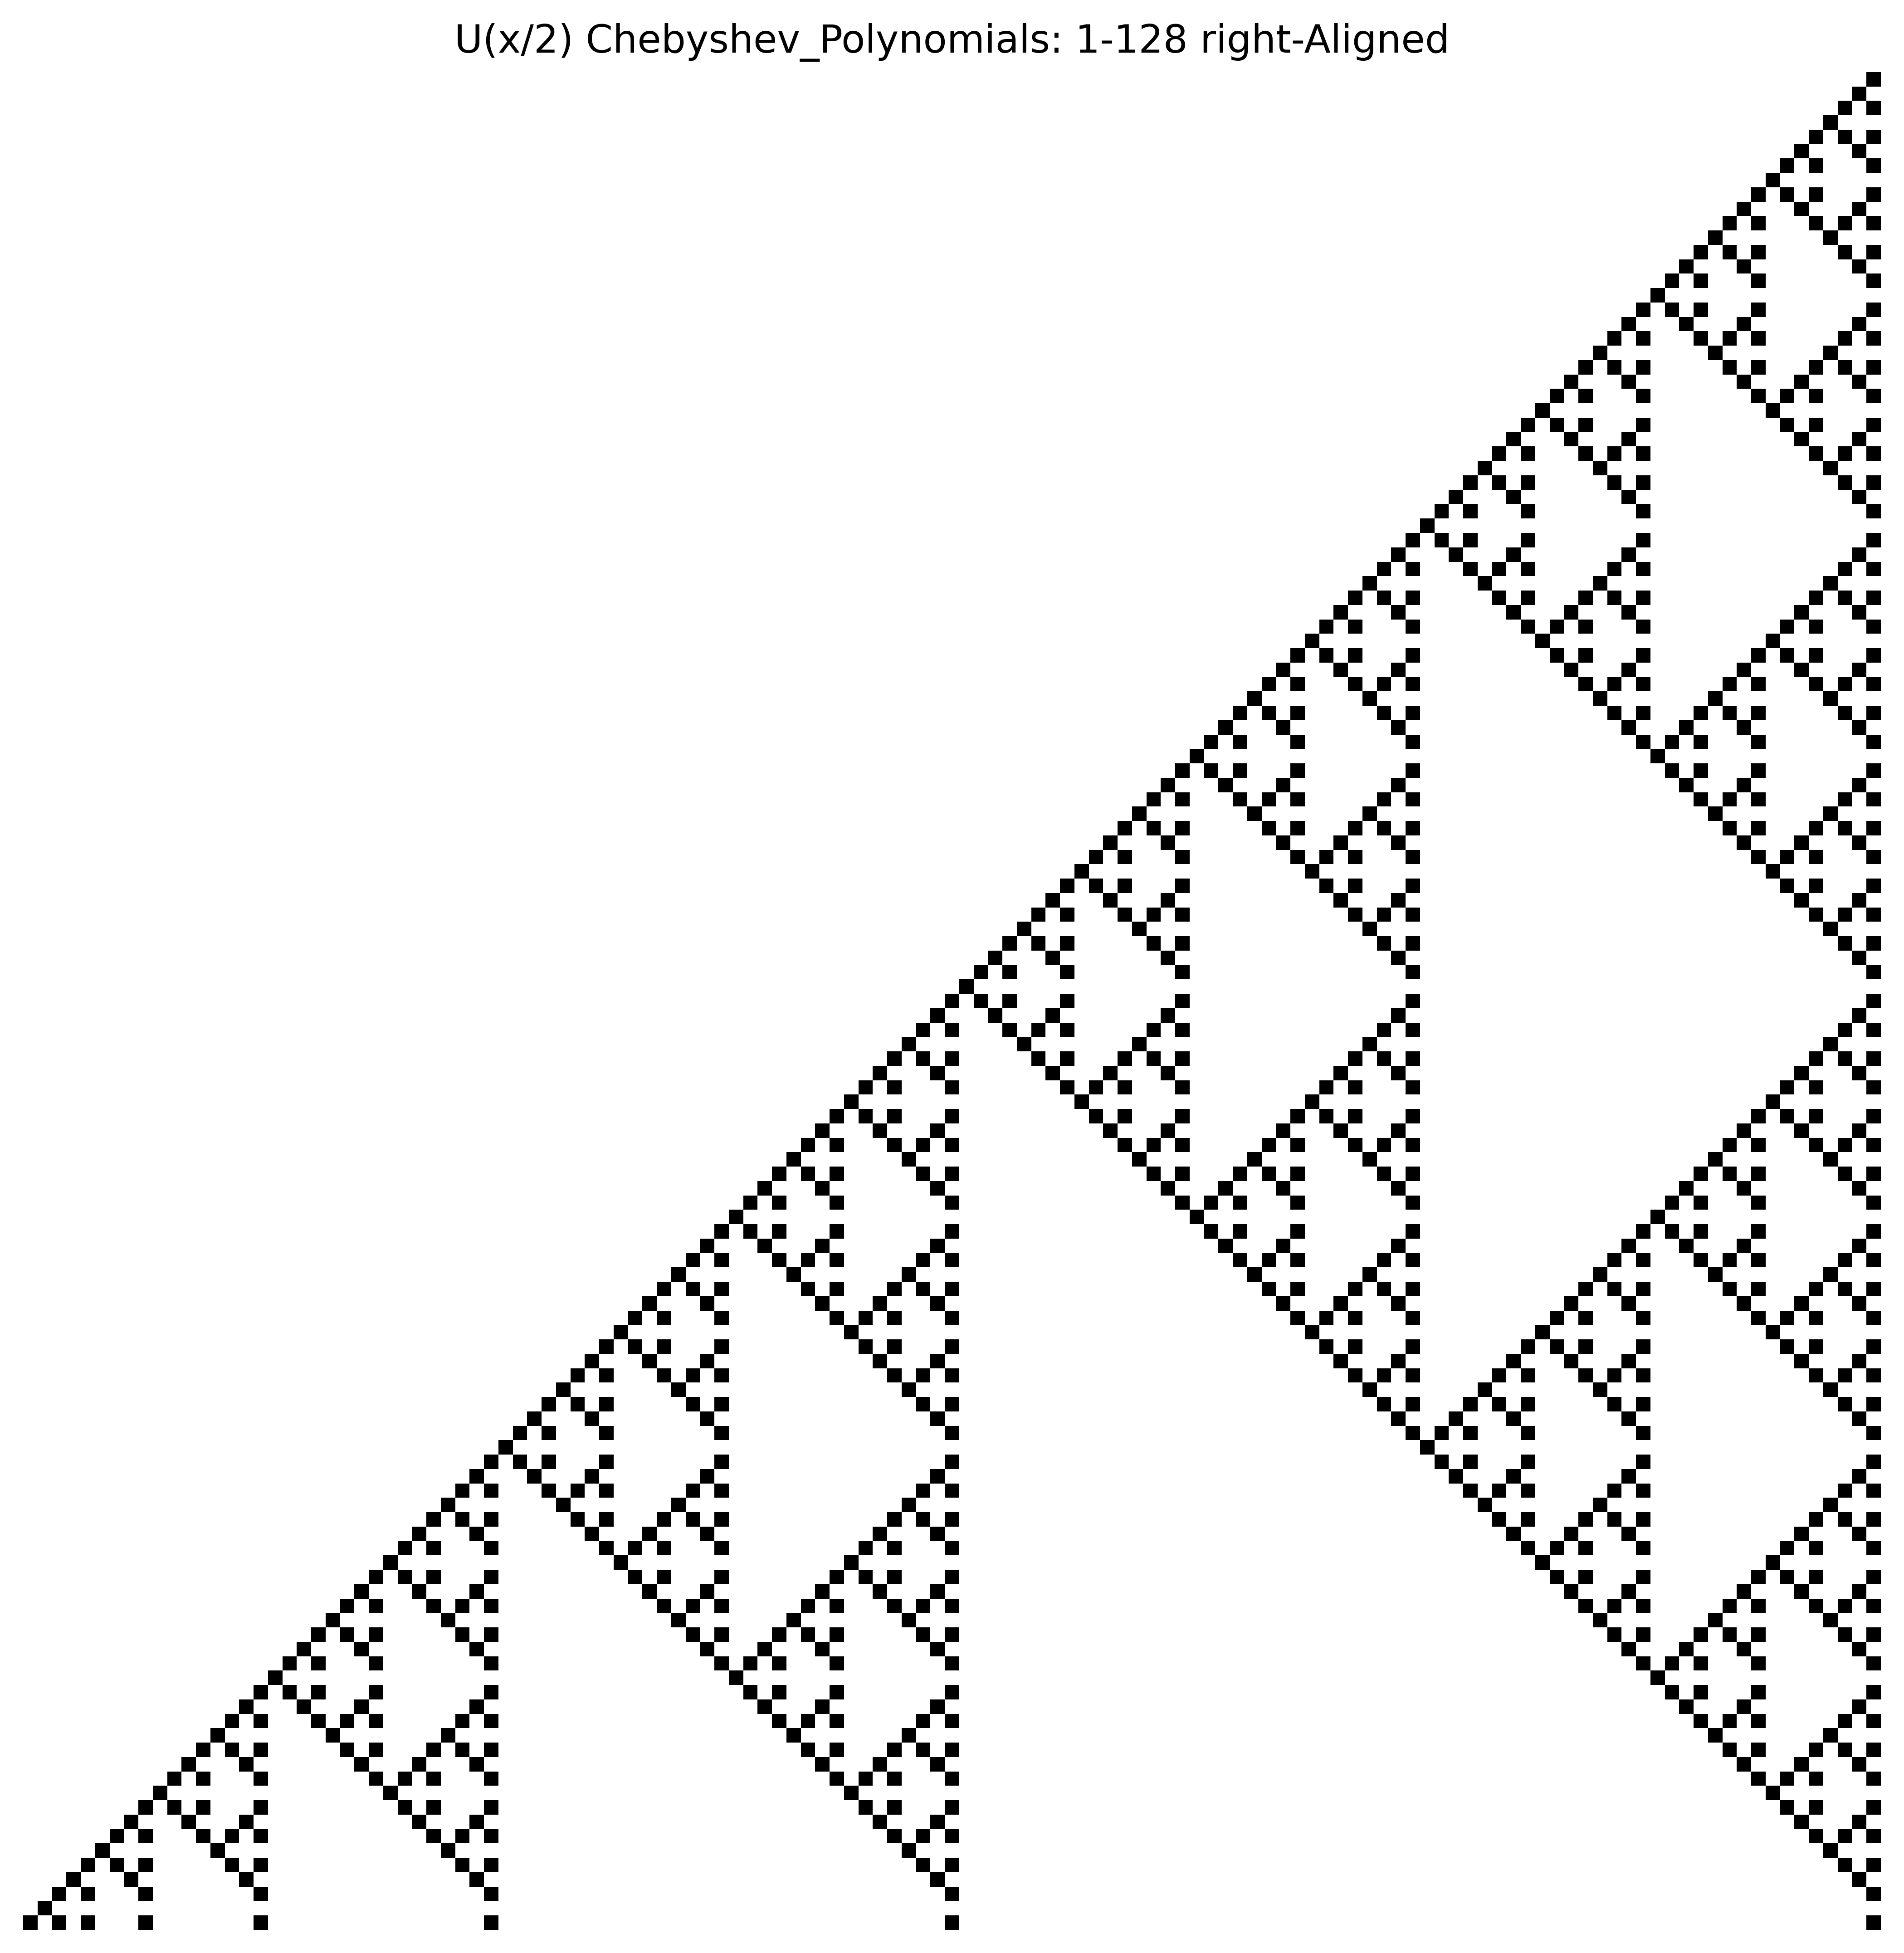
\includegraphics[width=.8\textwidth]{./chebyshev1_right_128.png}	
		\caption{$F_1(x)$ through $F_{128}(x)$, right-aligned.}
	\end{figure}
	
	Using a well-known connection between the Sierpinski triangle and the parity of binomial coefficients, we may see that
	\begin{equation*}
		F_n(x) = \sum_{i=0}^{n-1}{\binom{n+i}{2i+1}x^i \mod 2}.
	\end{equation*}

	The above construction and formula was also shown by Sutner \cite{Sutner96sigma-automataand}.
	Sutner also showed the following relationship between square \textit{Lights Out} grids and Fibonacci Polynomials.
	\begin{lemma}[Sutner]\label{FibonacciPolynomialGCD}
		Let $G = (V,E)$ be an $n \times m$ grid graph.
		Let $\Phi_G: P(V) \rightarrow P(V)$ be the function that maps which lights are clicked to which lights change state.
		Then
		\begin{equation*}
			\dim{\ker{\Phi_G}}
			= \deg{\left(\gcd{\left(F_{n+1}(x), F_{m+1}(x+1)\right)}\right)}
			= \deg{\left(\gcd{\left(F_{n+1}(x+1), F_{m+1}(x)\right)}\right)}.
		\end{equation*}
	\end{lemma}
	\begin{proof}See \cite{Sutner96sigma-automataand} theorem 5.1.\end{proof}
	
	Sutner and others also shows several divisibility rules for these polynomials
	\begin{lemma}[Hunziker, Machiavelo, and Park]\label{FibonacciDivisibility}
		A polynomial $\tau(x)$ in $\F_2[x]$ divides both $F_n(x)$ and $F_m(x)$ if and only if it divides $F_{\gcd(m,n)}(x)$.
		In particular,
		\begin{equation*}
			\gcd{\left(F_m(x),F_n(x)\right)} = F_{\gcd(m,n)}(x).
		\end{equation*}
	\end{lemma}
	\begin{proof}
		See \cite{HUNZIKER2004465} proposition 2.2, \cite{Sutner96sigma-automataand} proposition 2.1, and \cite{Knuth_AOCP4A}.
	\end{proof}
	% TODO: Check Knuth citation. It may be a different set of exercises.
	
	\begin{corollary}\label{Threeven}
		The following are true:
		\begin{enumerate}[label=(\roman*)]
			\item $x$ divides $F_n(x)$ if and only if $n \equiv 0 \mod 2$.
			\item $x+1$ divides $F_n(x+1)$ if and only if $n \equiv 0 \mod 2$.
			\item $x+1$ divides $F_n(x)$ if and only if $n \equiv 0 \mod 3$.
			\item $x$ divides $F_n(x+1)$ if and only if $n \equiv 0 \mod 3$.
		\end{enumerate}
	\end{corollary}
	\begin{proof}
		Notice,
		\begin{enumerate}[label=(\roman*)]
			\item
			We find that $f_2(x) = x$ is the smallest Fibonacci polynomial divisible by $x$, so we apply lemma \ref{FibonacciDivisibility} to get the desired result.
			\item
			Follows from (i) by substituting $x+1$ for $x$.
			\item
			We find that $f_3(x) = (x+1)^2$ is the smallest Fibonacci polynomial divisible by $x+1$, so we apply lemma \ref{FibonacciDivisibility} to get the desired result.
			\item
			Follows from (iii) by substituting $x+1$ for $x$.
		\end{enumerate}
	\end{proof}
	
	\begin{lemma}[Hunziker, Machiavelo, and Park]\label{SquareSquareFree}
		If $n$ is odd, then $F_n(x)$ is the square of a square-free polynomial.
	\end{lemma}
	\begin{proof}
		See \cite{HUNZIKER2004465} proposition 2.11 and \cite{Sutner96sigma-automataand} Theorem 2.1 claim 2.
	\end{proof}
	
	% TODO: Check is this proof is immediate
	\begin{corollary}
		If $n$ is odd, then every root of $F_n(x)$ has multiplicity 2.
	\end{corollary}
	\begin{proof}
		Let $n$ be odd and $\alpha$ a root of $F_n(x)$.
		By \ref{SquareSquareFree}, there exists $\tau_n \in \F_2[x]$ such that
		\begin{equation*}
			F_n(x) = \tau_n(x)^2,
		\end{equation*}
		and $\tau(x)$ is square-free.
		Since $\alpha$ is a root of $F_n(x)$, it must also be a root of $\tau_n(x)$ and thus has multiplicity 2.
	\end{proof}
	
	We can now prove some of our own facts about these polynomials and their GCDs, particularly on square grids.
	\begin{lemma}\label{DEven}
		Let $d(n) = \dim{\ker{\Phi_G}}$ for $G$ an $n \times n$ grid graph.
		Then $d(n)$ is always even.
	\end{lemma}
	\begin{proof}
		Let
		\begin{equation*}
			G_n(x) = \gcd{\left(F_{n}(x),F_{n}(x+1)\right)}.
		\end{equation*}
		By lemma \ref{FibonacciPolynomialGCD}, we know that $d(n) = \deg{G_{n+1}(x)}$ and $G_n(x) = G_n(x+1)$.
		
		$y = x(x+1)$ is also unchanged by this $x \mapsto x+1$ translation.
		It is well-know that every polynomial $P(x)$ in $\F_2[x]$ can be uniquely written as
		\begin{equation*}
			P(x) = A(y) + xB(y) \qquad A, B \in \F_2[y].
		\end{equation*}
		We can then determine exactly when $P$ is also unchanged by translation.
		\begin{align*}
			P(x+1) &= P(x) \\
			A(y)+(x+1)B(y) &= A(y) + xB(y) \\
			B(y) &= 0.
		\end{align*}
		In other words, $P(x)$ in unchanged by translation when $P$ is a polynomial in $x^2 + x$.
		
		Since $G_n$ is also unchanged by translation, there exists $H_n \in \F_2[x]$ such that
		\begin{equation*}
			G_n(x) = H_n(x^2 + x).
		\end{equation*}
		So,
		\begin{equation*}
			d(n) = \deg{G_{n+1}(x)} = 2\deg{H_{n+1}(x)}
		\end{equation*}
		and thus $d(n)$ is even.
	\end{proof}

	\begin{corollary}\label{NEvenDDivisible4}
		If $n$ is even, then $d(n)$ is divisible by 4.
	\end{corollary}
	\begin{proof}
		If $n$ is even, then $n+1$ is odd.
		Then by \ref{SquareSquareFree}, $F_{n+1}(x)$ and $F_{n+1}(x+1)$ are squares of square-free polynomials $\tau(x)$ and $\tau(x+1)$.
		\begin{align*}
			G_{n+1}(x) &= \gcd{\left(F_{n+1}(x),F_{n+1}(x+1)\right)} \\
			&= \gcd{\left(\tau_{n+1}(x)^2, \tau_{n+1}(x+1)^2\right)} \\
			&= \gcd{\left(\tau_{n+1}(x), \tau_{n+1}(x+1)\right)}^2 \\
			\sqrt{G_{n+1}(x)} &= \gcd{\left(\tau_{n+1}(x), \tau_{n+1}(x+1)\right)}
		\end{align*}
		We can see from the right-hand side of the equation that this function is also unaffected by translation.
		So, by lemma \ref{DEven}, there exists $H_{n+1} \in \F_2[x]$ such that
		\begin{align*}
			\sqrt{G_{n+1}(x)} &= H_{n+1}(x^2+x) \\
			G_{n+1}(x) &= H_{n+1}(x^2+x)^2.
		\end{align*}
		So,
		\begin{equation*}
			d(n) = \deg G_{n+1}(x) = 4\deg{H_{n+1}(x)},
		\end{equation*}
		as desired.
	\end{proof}
	Note that the implication does not hold in the other direction: $d(n)$ also be divisible by 4 when $n$ is odd.
	For example, $d(9) = 8$.

	\begin{lemma}\label{FibonacciFormulaT}
		Let $x = t + t^{-1}$.
		Then for $t \neq 0$,
		\begin{equation*}
			xF_n(x) = t^{n} + t^{-n}.
		\end{equation*}
	\end{lemma}
	\begin{proof}
		Define $G_n(t) = t^{n+1} + t^{-(n+1)}$.
		Then
		\begin{align*}
			xG_{n-1}(t) + G_{n-2}(t) &= (t+t^{-1})(t^{n}+t^{-n}) + (t^{n-1}+t^{-(n-1)}) \\
			&= t^{n+1} + t^{-(n-1)} + t^{n-1} + t^{-(n+1)} + t^{n-1} + t^{-(n-1)} \\
			&= t^{n+1} + t^{-(n+1)} \\
			&= G_n.
		\end{align*}
		Thus we see that $G_n(t)$ satisfies the same recurrence relation as $F_n(x)$.
		$xF_n(x)$ also satisfies the same recurrence relation.
		\begin{align*}
			xF_n(x) &= x(xF_{n-1}(x)+F_{n-2}(x)) \\
			&= x(xF_{n-1}(x)) + xF_{n-2}(x).
		\end{align*}
		Now we compute $xF_1(x)$ and $xF_2(x)$ in terms of $t$ and $G$:
		\begin{align*}
			xF_1(x) &= x \\
			&= t + t^{-1} \\
			&= G_0(t),
		\end{align*}
		and
		\begin{align*}
			xF_2(x) &= x^2 \\
			&= (t+t^{-1})^2 \\
			&= t^2 + t^{-2} \\
			&= G_1(t).
		\end{align*}
		Since the first two terms match and they satisfy the same recurrence relation then we've shown by induction that for $t \neq 0$,
		\begin{equation*}
			xF_n(x) = G_{n-1}(t) = t^{n} + t^{-n}.
		\end{equation*}
	\end{proof}
	This was also proven in \cite{HUNZIKER2004465}, who also prove the following identities.
	
	\begin{lemma}[Hunziker, Machiavelo, and Park]\label{Fibonacci2k}
		Let $n = 2^k b$ where $b,k \in \N$.
		Then
		\begin{equation*}
			F_n(x) = x^{2^k-1}F_b(x)^{2^k}.
		\end{equation*}
	\end{lemma}
	\begin{proof}
		See \cite{HUNZIKER2004465} lemma 2.6.
	\end{proof}

	\begin{lemma}\label{RootParameterization}
		The distinct roots of $F_n(x)$ are $\{\zeta + \zeta^{-1} : \zeta^{n} = 1, \zeta \neq 1\}$, plus 0 when $n$ is even.
	\end{lemma}
	\begin{proof}
		Notice that $F_n(0) = F_{n-2}(0)$, so
		\begin{equation*}
			F_n(0) = \begin{cases}
				1 & n \text{ odd} \\
				0 & n \text{ even}
			\end{cases}.
		\end{equation*}
		Thus 0 is a root of $F_n(x)$ whenever $n$ is even.
		
		Let $\alpha$ be a non-zero root of $F_n$.
		Choose $\zeta$ satisfying
		\begin{equation*}
			\zeta^2 + \alpha\zeta + 1 = 0.
		\end{equation*}
		Notice that $\zeta$ cannot be 0.
		Dividing by $\zeta$,
		\begin{align*}
			\zeta + \alpha + \zeta^{-1} &= 0 \\
			\alpha &= \zeta + \zeta^{-1}.
		\end{align*}
		By, Lemma \ref{FibonacciFormulaT},
		\begin{align*}
			0 &= \alpha F_n(\alpha) \\
			&= \zeta^{n} + \zeta^{-n} \\
		\end{align*}
		Since a field has no nonzero nilpotents, we may multiply by $\zeta^n$.
		\begin{align*}
			0 &= \zeta^{2n} + 1 \\
			&= \left(\zeta^{n}+1\right)^2 \\
			&= \zeta^{n} + 1 \\
			\zeta^{n} &= 1.
		\end{align*}
		Thus the order of $\zeta$ divides $n$.
		Notice too that $\zeta \neq 1$; otherwise, $\alpha = 1 + 1^{-1} = 0$, which we already showed as not possible.
		
		Conversely, if $\zeta^{n} = 1$ and $\zeta \neq 1$, then let $\alpha = \zeta + \zeta^{-1}$.
		Then we see $\alpha \neq 0$ and
		\begin{equation*}
			\alpha F_n(\alpha) = \zeta^{n} + \zeta^{-n} = 1 + 1^{-1} = 0.
		\end{equation*}
		Thus, $\alpha$ is a root of $F_n$.
	\end{proof}

	\section{Even Parity Covers}
	$\ker{\Phi_G}$ may also be understood via parity covers and dominating sets.
	
	\begin{definition}
		An \textit{even dominating set} of a graph $G = (V,E)$ is a subset $V' \subseteq V$ such that every vertex contains an even number of vertices from $V'$ in its neighborhood. 
	\end{definition}
	Odd dominating sets can be analogously defined.
	Sutner specifically studied odd dominating sets as the solution to \textit{Lights Out} when all lights are initially on.
	He showed that such an odd dominating set always exists for any finite graph \cite{Sutner1989}.
	
	\begin{lemma}
		$V' \in \ker{\Phi_G}$ if and only if $V'$ is an even dominating set of $G$.
	\end{lemma}
	\begin{proof}
		Let $V' \in \ker{\Phi_G}$.
		Let $N(v)$ be the neighborhood of vertex $v$: $v$ and its immediate neighbors.
		Then for every $v \in V$,
		\begin{equation*}
			\abs{N(v) \cap V'} \text{ is even}.
		\end{equation*}
		Thus, $V'$ is an even dominating set of $G$.
		We can apply the same steps in reverse to show the converse.
	\end{proof}

	% TODO: Find a reference for this
	\begin{lemma}
		$\Phi_G$ is linear with respect to symmetric difference.
		That is, for all $V_1, V_2 \subseteq V$,
		\begin{equation*}
			\Phi_G(V_1 \triangle V_2) = \Phi_G(V_1) \triangle \Phi_G(V_2).
		\end{equation*}
	\end{lemma}
	\begin{proof}
		\begin{align*}
			\Phi_G(V_1 \triangle V_2) &= \{v \in V : \abs{N(v) \cap (V_1 \triangle V_2)} \text{ is odd}\} \\
			&= \left(\{v \in V : \abs{N(v) \cap V_1} \text{ is odd}\} \cup \{v \in V : \abs{N(v) \cap V_2} \text{ is odd}\}\right) \setminus \{v \in V : \abs{N(v) \cap (V_1 \cap V_2)} \text{ is odd}\} \\
			&= \{v \in V : \abs{N(v) \cap V_1} \text{ is odd}\} \triangle \{v \in V : \abs{N(v) \cap V_2} \text{ is odd}\} \\
			&= \Phi_G(V_1) \triangle \Phi_G(V_2)
		\end{align*}
	\end{proof}
	% TODO: An AI review said this proof wasn't entirely correct. Double check.

	\begin{corollary}
		If $V_1$ and $V_2$ have the same image under $\Phi_{G}$ if and only if $V_1 \triangle V_2 \in \ker{\Phi_G}$.
	\end{corollary}
	\begin{proof}
		Assume that $V_1$ and $V_2$ have the same image under $\Phi_G$.
		Then
		\begin{align*}
			\Phi_{G}(V_1 \triangle V_2) &= \Phi_{G}(V_1) \triangle \Phi_{}(V_2) \\
			&= \Phi_{G}(V_1) \triangle \Phi_{G}(V_2) \\
			&= \emptyset.
		\end{align*}
		Thus, $V_1 \triangle V_2 \in \ker{\Phi_G}$.
		Now assume $V_1 \triangle V_2 \in \ker{\Phi_G}$.
		Then
		\begin{align*}
			\Phi_G(V_1) &= \Phi_G(V_1) \triangle \emptyset \\
			&= \Phi_{G}(V_1) \triangle \Phi_{G}(V_1 \triangle V_2) \\
			&= \Phi_{G}(V_1) \triangle \Phi_{G}(V_1) \triangle \Phi_{G}(V_2) \\
			&= \Phi_{G}(V_2).
		\end{align*}
		Thus $V_1$ and $V_2$ have the same image under $\Phi_G$.
	\end{proof}
	
	We may now use our geometric understanding of $\ker{\Phi_G}$ as even parity covers to construct a lower bound on $d(n)$.
	\begin{theorem}
		For all $n,k \in \N$,
		\begin{equation*}
			d(nk-1) \geq d(n-1).
		\end{equation*}
	\end{theorem}
	\begin{proof}
		Let $G_L$ be an $nk-1 \times nk-1$ grid and $G_\ell$ be an $n-1 \times n-1$ grid.
		Since $nk-1 = k(n-1) + (k-1)$, an $G$ may be broken into a $k \times k$ grid of $n-1 \times n-1$ grids, each separated by a horizontal or vertical strip of size 1.
		
		Let $Q$ be an even dominating set of $G_\ell$.
		Let $R$ be $Q$ tiles $k$ times horizontally and vertically, with size 1 separators between each tile, onto $G_L$ where each tile is the reflection across its neighboring separators, as shown below.
		
		\begin{figure}[H]
			\centering
			% Code the generate figure w/o Q's
			%			\begin{tikzpicture}[scale=0.33]
				%				\edef\M{3} % Width of each tile
				%				\edef\K{5} % Number of tiles in each direction
				%				\pgfmathparse{(\M+1)*\K - 1} % Size of large grid
				%				\edef\N{\pgfmathresult}
				%				
				%				\draw[black,thin] (0,0) grid (\N,\N);
				%				
				%				\foreach \i in {1,2,...,\K}{
					%					\foreach \j in {1,2,...,\K}{
						%						\pgfmathparse{(\i - 1) * (\M + 1)}
						%						\edef\X{\pgfmathresult}
						%						\pgfmathparse{(\j - 1) * (\M + 1)}
						%						\edef\Y{\pgfmathresult}
						%						
						%						\draw[fill,gray,opacity=0.707] (\X, \Y) rectangle (\X + \M, \Y + \M);
						%						%\node at (\X + \M/2, \Y + \M/2) {$Q$};
						%					}
					%				}
				%			\end{tikzpicture}
			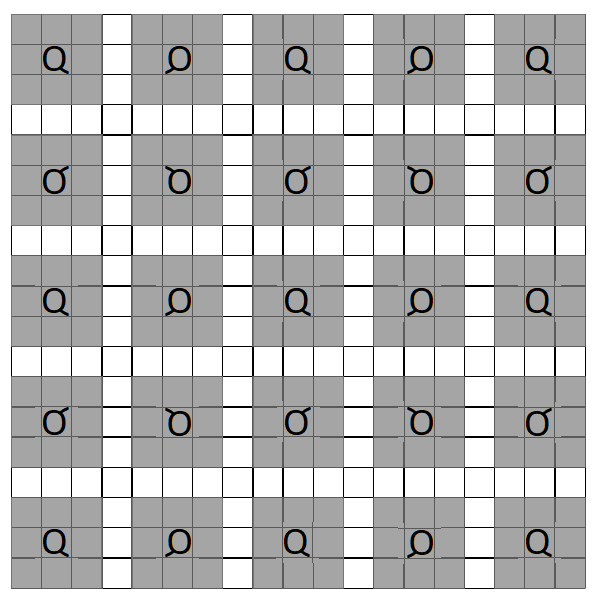
\includegraphics[width=0.5\textwidth]{tiling_q.png}
			\caption{Pattern $Q$ tiled 5 times.}	
		\end{figure}
	
		Consider an vertex $v$ in $G_L$.
		There are 3 cases.
		\begin{enumerate}
			\item
				$v$ is within a tile.
				Then $\abs{N(v) \cap R}$ is even because $Q$ being is an even parity cover.
			\item
				$v$ is on a separator between two tiles.
				Then only two elements in $N(v)$, the vertices within a tile, are also in $R$.
				Because neighboring tiles are reflections of each other across separators, these two vertices are either both in $R$ or both not in $R$.
				In either case, $\abs{N(v) \cap R}$ is even.
			\item
				$v$ is in the intersection of two separators.
				Then all of $N(v)$ is in a separator and thus not in $R$, so $\abs{N(v) \cap R} = 0$, which is even.
		\end{enumerate}
		Since for every vertex $v$ of $G_L$, $\abs{N(v) \cap R}$ is even, so $R$ is an even dominating set of $G_L$.
		Thus, for every even dominating set of $G_\ell$, there exists an even dominating set of $G_L$ obtained through tiling.
		This tiling function is also injective because we can recover $Q$ by restricting $R$ to just the top left tile.
		Thus,
		\begin{equation*}
			d(nk-1) \geq d(n-1),
		\end{equation*}
		as desired.
	\end{proof}
	Sutner shows a similar result \cite{Sutner1988_2}.
	There is also a simple proof in terms of Fibonacci polynomials that also provides a divisibility relationship.
	\begin{proof}
		Since $n$ divides $nk$, lemma \ref{FibonacciDivisibility} tells us $F_{n}(x)$ divides $F_{nk}(x)$.
		So,
		\begin{equation*}
			\gcd{\left(F_n(x),F_n(x+1)\right)} \mid \gcd{\left(F_{nk}(x),F_{nk}(x+1)\right)}.
		\end{equation*}
		So we may write
		\begin{equation*}
			\gcd{\left(F_{nk}(x),F_{nk}(x+1)\right)} = 	\gcd{\left(F_n(x),F_n(x+1)\right)} Q(x),
		\end{equation*}
		for some $Q(x) \in \F_2[x]$.
		Taking the degrees, we obtain $d(nk-1) = d(n-1) + \deg{Q(x)}$, and so the desired inequality follows.
	\end{proof}
	Note that although the smaller GCD polynomial divides the larger, it's not the case that $d(n-1)$ divides $d(nk-1)$.
	For example, if $n=5$ and $k=6$, then $d(n-1) = d(4) = 4$, which does not divide $d(nk-1) = d(29) = 10$.

	\section{Number Theory}
	We may also understand $d(n)$ and the Fibonacci polynomials with some results from number theory.
	
	\begin{lemma}[Ore]\label{OreGcd}
		Let $a$, $b$, $c$, and $d$ be integers.
		Let $(a,b)$ denote $\gcd{(a,b)}$.
		Then
		\begin{equation*}
			(ab,cd) = (a,c)(b,d)\left(\frac{a}{(a,c)},\frac{d}{(b,d)}\right)\left(\frac{c}{(a,c)},\frac{b}{(b,d)}\right).
		\end{equation*}
	\end{lemma}
	\begin{proof}
		See \cite{ore_number_theory}.
	\end{proof}
	Although Ore's result deals specifically with integers, both the integers and $\F_2[x]$ are Euclidean domains, so the result will still hold for our purposes.
	
	\begin{theorem}\label{2nPlus1}
		For all $n \in \N$,
		\begin{equation*}
			d(2n+1) = 2d(n) + \delta_n, \qquad
			\delta_n = \begin{cases}
				2 & 3 \mid n+1 \\
				0 & \text{otherwise}
			\end{cases}.
		\end{equation*}
	\end{theorem}
	\begin{proof}
		Let $(a,b)$ denote $\gcd{(a,b)}$.
		Applying lemmas \ref{Fibonacci2k} and \ref{OreGcd},
		% TODO: Some of these equations run off the page
		\begin{align*}
			d(2n+1) &= \deg{\left(F_{2n+2}(x),F_{2n+2}(x+1)\right)} \\
			&= \deg{\left(xF_{n+1}(x)^2,(x+1)F_{n+1}(x+1)^2\right)} \\
			&= \deg{(x,x+1)\left(F_{n+1}(x)^2,F_{n+1}(x+1)^2\right)\left(\frac{x+1}{(x,x+1)},\frac{F_{n+1}(x)^2}{\left(F_{n+1}(x)^2,F_{n+1}(x+1)^2\right)}\right)\left(\frac{x}{(x,x+1)},\frac{F_{n+1}(x+1)^2}{\left(F_{n+1}(x)^2,F_{n+1}(x+1)^2\right)}\right)} \\
			&= \deg{\left(F_{n+1}(x),F_{n+1}(x+1)\right)^2\left(x+1,\frac{F_{n+1}(x)^2}{\left(F_{n+1}(x),F_{n+1}(x+1)\right)^2}\right)\left(x,\frac{F_{n+1}(x+1)^2}{\left(F_{n+1}(x),F_{n+1}(x+1)\right)^2}\right)} \\
			&= 2d(n) + 2\deg{\left(x,\frac{F_{n+1}(x+1)^2}{\left(F_{n+1}(x),F_{n+1}(x+1)\right)^2}\right)}
		\end{align*}
		Thus, we have that
		\begin{equation*}
			\delta_n = 2\deg{\left(x,\frac{F_{n+1}(x+1)^2}{\left(F_{n+1}(x),F_{n+1}(x+1)\right)^2}\right)}.
		\end{equation*}
		So, $\delta_n$ is 2 exactly when $F_{n+1}(x)$ can be divided without remainder by $x+1$ more times than $F_{n+1}(x+1)$.
		When $n+1$ is not divisible by 3, corollary \ref{Threeven} tells us that $F_{n+1}(x)$ is not divisible by $x+1$, so $\delta_n = 0$.
		When $n+1$ is divisible by 3, let $n+1 = b 2^{k}$ for $b,k \geq 0$ and $b$ odd.
		Then $b$ must be divisible by 3.
		Applying Lemma \ref{Fibonacci2k},
		\begin{equation*}
			F_{n+1}(x) = x^{2^{k}-1}F_{b}(x)^{2^k} \qquad F_{n+1}(x+1) = (x+1)^{2^{k}-1}F_{b}(x+1)^{2^k}.
		\end{equation*}
		Since $b$ is an odd multiple of 3, corollary \ref{Threeven} tells us that $x+1$ divides $F_{b}(x)$, but $x+1$ does not divide $F_b(x+1)$.
		So,
		\begin{equation*}
			F_{n+1}(x) = x^{2^{k}-1}(x+1)^{2^k}g(x)^{2^k} \qquad F_{n+1}(x+1) = (x+1)^{2^{k}-1}x^{2^k}g(x+1)^{2^k},
		\end{equation*}
		for some $g(x) \in \F_2[x]$, where $g(x)$ and $g(x+1)$ are both divisible by neither $x$ nor $x+1$.
		So, we see that $F_{n+1}(x)$ can be divided without remainder by $x+1$ more times than $f_{n+1}(x+1)$, so $\delta_n = 2$.
	\end{proof}
	This result resolves a conjecture of Sutner's \cite{Sutner1989}.
	
	% TODO: An AI review of the above proof flagged "(x+1) occurs with multiplicity (2) in odd" and "(F_b) when (3\mid b). Rewrite this part using valuations" but I'm not really sure what these mean.
	
	We can repeatedly apply theorem \ref{2nPlus1} to obtain explicit formulas for $d(n)$.
	\begin{corollary}\label{2nPlus1Explicit}
		Write odd $n$ as $n+1 = 2^s b$ for $s \geq 0$ and $b$ odd.
		Then
		\begin{equation*}
			d(n) = 2^s d(b-1) + \begin{cases}
				2(2^s - 1) & 3 \mid b \\
				0 & \text{otherwise}
			\end{cases}.
		\end{equation*}
	\end{corollary}
	\begin{proof}
		By induction on $s$.
		For $s=0$,
		\begin{align*}
			n+1 &= 2^0 b \\
			n &= b-1 \\
			d(n) &= d(b-1) \\
			&= 2^0 d(b-1) + \begin{cases}
				2(2^0 - 1) & 3 \mid b \\
				0 & \text{otherwise}
			\end{cases},
		\end{align*}
		as desired.
		Assume that our claim holds for $s \geq 0$.
		Then for $n+1 = 2^{s+1}b$,
		\begin{align*}
			d(n) &= d\left(2^{s+1}b - 1\right) \\
			&= d\left(2\left(2^s b - 1\right) + 1\right) \\
			&= 2d\left(2^s b - 1\right) + \begin{cases}
				2 & 3 \mid 2^s b \\
				0 & \text{otherwise}
			\end{cases} \\
			&= 2\left(2^s d(b-1) + \begin{cases}
				2(2^s - 1) & 3 \mid b \\
				0 & \text{otherwise}
			\end{cases}\right) + \begin{cases}
				2 & 3 \mid 2^s b \\
				0 & \text{otherwise}
			\end{cases} \\
			&= 2^{s+1}d(b-1) + \begin{cases}
				2(2^{s+1} - 1) - 2 & 3 \mid b \\
				0 & \text{otherwise}
			\end{cases} + \begin{cases}
				2 & 3 \mid b \\
				0 & \text{otherwise}
			\end{cases} \\
			&= 2^{s+1}d(b-1) + \begin{cases}
				2(2^{s+1} - 1) & 3 \mid b \\
				0 & \text{otherwise},
			\end{cases} 
		\end{align*}
		as desired.
	\end{proof}
	
	We can also use theorem \ref{2nPlus1} to narrow down more when $d(n) = 2$.
	\begin{corollary}\label{D2Minus1Mod6}
		If $d(n) = 2$, then $n \equiv -1 \pmod 6$.
	\end{corollary}
	\begin{proof}
		Since 2 is not divisible by 4, corollary \ref{NEvenDDivisible4} tells us that $n$ must be odd.
		So, we can write $n = 2^k b - 1$ for $b$ odd and $k \geq 1$.
		Using corollary \ref{2nPlus1Explicit}, we can define
		\begin{equation*}
			D_i = d(2^i b - 1) = \begin{cases}
				2^i d(b-1) + 2(2^i - 1) & 3 \mid b \\
				2^i d(b-1) & \text{otherwise}
			\end{cases}.
		\end{equation*}
		If $3 \nmid b$, then we must have $D_k = 2 = 2^k d(b-1)$.
		However, corollary \ref{NEvenDDivisible4} tells us that $d(b-1)$ is divisible by 4, which cannot be the case.
		
		If $3 \mid b$, then we must have $D_k = 2 = 2^k d(b-1) + 2(2^k - 1)$.
		If $k \geq 2$, then this expression is greater than 2, which cannot be the case.
		Thus, we must have $k=1$ and $D_1 = 2 = 2 d(b-1) + 2$, which simplifies to $d(b-1) = 0$.
		Thus we may write $b = 3j$.
		
		Solving for $n$, we find
		\begin{align*}
			n &= 2^k b - 1 \\
			&= 2b - 1 \\
			&= 6j - 1,
		\end{align*}
		so $n \equiv -1 \pmod 6$, as desired.
	\end{proof}
	
	% TODO: We may also need to show a lemma that if rank(P) is the least r such that P divides F_r, then P divides F_m if and only if rank(P) divides m.
	
	We can now use this recurrence result to prove the impossibility of certain values of $d(n)$.
	\begin{theorem}
		The smallest even $k$ such that for all $n \in \N$, $d(n) \neq k$ is $k=26$.
	\end{theorem}
	\begin{proof}
		Recall from lemma \ref{DEven} that $d(n)$ is always even.
		Through calculation, we can find that
		\begin{alignat*}{12}
			d(5) &= 2 \qquad & d(4) &= 4 \qquad & d(11) &= 6 \qquad & d(16) &= 8 \qquad & d(29) &= 10 \qquad & d(84) &= 12 \\
			d(23) &= 14 \qquad & d(19) &= 16 \qquad & d(101) &= 18 \qquad & d(30) &= 20 \qquad & d(59) &= 22 \qquad & d(62) &= 24.
		\end{alignat*}
		We will show than $d(n)=26$ is impossible.
		
		Assume for the sake of contradiction that there exists $n \in \N$ such that $d(n) = 26$.
		Since 26 is not divisible by 4, corollary \ref{NEvenDDivisible4} that $n$ must be odd.
		So, we may write $n = 2m+1$.
		By theorem \ref{2nPlus1},
		\begin{equation*}
			26 = d(n) = d(2m+1) = 2d(m) + \begin{cases}
				2 & 3 \mid m+1 \\
				0 & \text{otherwise}
			\end{cases}.
		\end{equation*}
		Since lemma \ref{DEven} tells us that $d(m)=13$ is not possible, we must have $d(m) = 12$ and $m+1$ is divisible by 3.
		Let $m+1 = 2^s b$ for odd $b$ and $s \geq 0$.
		By corollary \ref{2nPlus1Explicit},
		\begin{equation*}
			d(m) = 2^s d(b-1) + 2(2^s - 1) = 12.
		\end{equation*}
		The only possible integer solutions here are $d(b-1)=12$ and $s=0$ or $d(b-1)=5$ and $s=1$.
		Since lemma \ref{DEven} tells us that $d(b-1) = 5$ is impossible, the only remaining possibility is that $d(m) = d(b-1) = 12$ and $s=0$.
		Thus, $m$ must be even.
		
		We know from lemma \ref{FibonacciPolynomialGCD} that
		\begin{equation*}
			d(m) = \deg{\left(\gcd{\left(F_{m+1}(x),F_{m+1}(x+1)\right)}\right)}.
		\end{equation*}
		Since $m+1$ is odd lemma \ref{SquareSquareFree} tells us that there exists some square-free $R_{m+1}(x)$ such that
		\begin{equation*}
			F_{m+1}(x) = R_{m+1}(x)^2.
		\end{equation*}
		Define $H_{m+1}(x)$
		\begin{equation*}
			H_{m+1}(x) = \gcd{\left(R_{m+1}(x),R_{m+1}(x+1)\right)} \qquad \gcd{\left(F_{m+1}(x),F_{m+1}(x+1)\right)} = H(x)^2.
		\end{equation*}
		Since $R_{m+1}(x)$ is square-free, then $H_{m+1}(x)$ is too.
		Since $d(m) = 12$, $\deg H_{m+1}(x) = 6$.
		Notice too that $H_{m+1}(x) = H_{m+1}(x+1)$, so our work in lemma \ref{FibonacciFormulaT} tells us that for $y = x^2 + x$, there exists square-free a cubic polynomial $h_{m+1}(y) \in \F_2[y]$ such that
		\begin{equation*}
			H_{m+1}(x) = h_{m+1}(y).
		\end{equation*}
		There are only three possible square-free cubic polynomials in $\F_2[y]$ that are also 1 at $y=0$:
		\begin{enumerate}
			\item $C_1(y) = y^3 + 1$
			\item $C_2(y) = y^3 + y + 1$
			\item $C_3(y) = y^3 + y^2 + 1$.
		\end{enumerate}
		We will handle these case-by-case.
		
		Define the ``$\operatorname{rank}$" of a polynomial $P$ to be the smallest integer $r$ such that $P$ divides $F_{r}$.
		Calculating the rank of our three candidates for $h_{m+1}(x)$,
		\begin{align*}
			\operatorname{rank}{\left((x^2+x)^3 + 1\right)} &= 85 \\
			\operatorname{rank}{\left((x^2+x)^3 + (x^2+x) + 1\right)} &= 63 \\
			\operatorname{rank}{\left((x^2+x)^3 + (x^2+x)^2 + 1\right)} &= 63
		\end{align*}
		If either rank-63 polynomials $C_2$ or $C_3$ divides $R_{m+1}(x)$, then 63 divides $m+1$.
		However, by definition of rank, both polynomials would divide $R_{m+1}(x)$.
		$C_2$ and $C_3$ are coprime and each of degree 6 in $x$, so $\deg H_{m+1}(x) = \deg{C_2(x)} + \deg{C_3(x)} = 12$, contradicting our assumption that the degree was 6.
		If $C_1$ $R_{m+1}$, then 85 divides $m+1$.
		Combining this with the fact that 3 divides $m+1$ we showed earlier, we see that 255 must divide $m+1$.
		
		Define
		\begin{equation*}
			P(x) = x^4 + x^3 + 1 \qquad Q(x) = x^4 + x^3 + x^2 + x + 1.
		\end{equation*}
		$P$ and $Q$ are coprime to each other and $C_1$.
		The ranks of $P(x)$ and $Q(x)$ are 15 and 17 respectively.
		Since both 15 and 17 divide 255, and 255 divides $m+1$, then both $P(x)$ and $Q(x)$ must divide $H_{m+1}(x)$.
		Therefore,
		\begin{equation*}
			\deg{H_{m+1}(x)} \geq \deg{C_1(x)} + \deg{P(x)} + \deg{Q(x)} = 14,
		\end{equation*}
		which contradicts our assumption that the degree was 6.
		
		Thus, there is no $3 \mid m+1$ such that $d(m) = 12$ and therefore no $n$ such that $d(n) = 26$.
	\end{proof}


	Now that we know that one impossible even value of $d(n)$ exists, we can show an entire family of impossible even values also exists.
	\begin{corollary}
		Suppose $a \in \N$ is even and an impossible value of $d(n)$.
		Then $2a+2$ is also an impossible value of $d(n)$.
	\end{corollary}
	\begin{proof}
		Suppose for the sake of contradiction that there exists $n$ such that $d(n) = 2a+2$.
		Since $2a+2$ is not divisible by 4, then corollary \ref{NEvenDDivisible4} tells us that n must be odd, so we may write $n = 2m+1$.
		So, by theorem \ref{2nPlus1},
		\begin{equation*}
			2a+2 = d(n) = d(2m+1) = 2d(m) + \delta_m \qquad \delta_m = \begin{cases}
				2 & 3 \mid m+1 \\
				0 & \text{otherwise}
			\end{cases}.
		\end{equation*}
		If $\delta_m = 0$, then $2d(m)$ is divisible by 4, which cannot be the case since we know the value is $2a+2$.
		If $\delta_m = 2$, then $d(m)=a$, contradicting the impossibility of $a$ as an output of $d$.
	\end{proof}
	Expanding the recurrence, if $a$ is an impossible value, then $2^t(a+2)-2$ is also impossible for all $t \geq 0$.
	In other words, 26, 54, 110, 222, 446, ... are also all impossible values of $d(n)$.
	
	\section{Finite Fields}
	Although we have already been working in $\F_2$, we will now more directly use results from the study of finite fields.
	
	\begin{lemma}\label{ordpj2}
		Let $p$ be an odd prime.
		Define $h = \ord[p]{2}$ and $c = v_p(2^h - 1)$, where
		$v_p(a)$ is the $p$-adic valuation of $a$.
		Then for every $j \geq 1$,
		\begin{equation*}
			\ord[p^j]{2} = h p^{\max{(0, j - c)}}.
		\end{equation*}
	\end{lemma}
	\begin{proof}
		Suppose $2^r \equiv 1 \pmod{p^j}$.
		Then $h$ divides $r$, so we may write $r = ht$.
		By the Lifting the Exponent Lemma,
		\begin{align*}
			v_p(2^r - 1) &= v_p(2^{ht} - 1) \\
			&= v_p(2^h - 1) + v_p(t) \\
			&= c + v_p(t).
		\end{align*}
		So, $p^j \mid 2^{ht} - 1$ exactly when $c + v_p(t) \geq j$.
		The smallest possible $t$ satisfying this inequality is $t = \max{(0, j-c)}$, so
		\begin{equation*}
			\ord[p^j]{2} = h p^{\max{(0, j-c)}},
		\end{equation*}
		as desired.
	\end{proof}
	% TODO: Do we need a citation for the lifting the exponent lemma?
	% Maybe Ireland & Rosen: A classical introduction to modern number theory chapter 2 (ss 2.7)?

	\begin{corollary}
		Let $p$ be an odd prime.
		If $p$ isn't a Wieferich prime, then
		\begin{equation*}
			\ord[p^j]{2} = \ord[p]{2} p^{j-1}.
		\end{equation*}
	\end{corollary}
	\begin{proof}
		Lemma \ref{ordpj2} tells us that
		\begin{equation*}
			\ord[p^j]{2} = \ord[p]{2} p^{\max{(0, j-c)}}, \qquad c = v_p(2^{\ord[p]{2}} - 1).
		\end{equation*}
		Thus it is sufficient to show that $c=1$.
		By definition of $\ord[p]{2}$, $c \geq 1$.
		Since $p$ is not a Wieferich prime, for all $t \geq 2$,
		\begin{equation*}
			p^{t} \nmid 2^{\ord[2]{p}} - 1,
		\end{equation*}
		so $c \ngeq 2$ and therefore must be exactly 1, as desired.
	\end{proof}
	% TODO: The standard definition of Wieferich prime is p^2 \mid 2^{p-1} - 1. Our proof uses p^2 \mid 2^{\ord[p]{2}} - 1.
	% This is equivalent by a lifting the exponent argument: If n = \ord[p]{a}, then p-1 = k*n, and a^(p-1) - 1 = a^(kn) - 1.
	% So, v_p(a^(kn) - 1) = v_p(a^n - 1) + v_p(k).
	% However, k = (p-1)/n is smaller than p and thus not divisible by p, so v_p(k) = 0.
	% So, v_p(a^(p-1) - 1) = v_p(a^n - 1).
	% So, p^2 \mid a^(p-1) - 1 if and only if p^2 \mid a^{\ord[p]{a}} - 1.
	% Should we prehaps include this argument?
	
	\begin{definition}
		Let $b$ be coprime to $n$.
		Then ``signed order" of $a$ modulo $n$ is
		\begin{equation*}
			\rho_b(n) = \min{\{r > 0 : b^r \equiv \pm 1 \pmod{n}\}}.
		\end{equation*}
	\end{definition}
	This is also sometimes called the ``index" of $"\pm 1$ relative to $b$, written $\operatorname{ind}_{b}(\pm 1)$.
	
	\begin{lemma}\label{signedOrder}
		Let $H_j = \ord[p^j]{2}$.
		Then
		\begin{equation*}
			\rho_{2}{(p^j)} = \begin{cases}
				H_j / 2 & H_j \text{ is even} \\
				H_j & H_j \text{ is odd}
			\end{cases}.
		\end{equation*}
		Moreover, when $H_j$ is even,
		\begin{equation*}
			2^{H_j / 2} \equiv -1 \pmod{p^j}.
		\end{equation*}
	\end{lemma}
	\begin{proof}
		Assume $H_j$ is even.
		Then by definition of $H_j$,
		\begin{equation*}
			\left(2^{H_j / 2}\right)^2 \equiv 1 \pmod{p^j}.
		\end{equation*}
		Thus the only solutions are $2^{H_j / 2} \equiv \pm 1 \pmod{p^j}$.
		However, 1 cannot be a solution; otherwise, $H_j$ would not be minimal.
		So,
		\begin{equation*}
			2^{H_j / 2} \equiv -1 \pmod{p^j}.
		\end{equation*}
		Notice that if $r \leq H_j / 2$, and $2^r \equiv -1 \pmod{p^j}$, then $2^{2r} \equiv 1 \pmod{p^j}$; since $H_j$ is minimal, $H_j \leq 2r$.
		Thus to satisfy both constraints we must have $H_j / 2 = r$.
		
		Now assume $H_j$ is odd.
		Notice that by definition, 
		\begin{equation*}
			H_j = \ord[p^j]{2} = \min{\{h > 0 : 2^h \equiv 1 \pmod{p^j}\}},
		\end{equation*} 
		so smaller solutions can only be of the form $2^r \equiv -1 \pmod{p^j}$.
		Then $2^{2r} \equiv 1 \pmod{p^j}$, which means $H_j \mid 2r$, and since $H_j$ is odd, $H_j \mid r$.
		Thus $H_j \leq r$, so $H_j$ is minimal, as desired.
	\end{proof}
	
	We can use this notion of a signed order to find the extension degree of extensions of $\F_2$.
	\begin{lemma}\label{fieldExtensionSize}
		Let $M > 1$ be odd; let $\zeta$ have exact order $M$; set $\alpha = \zeta + \zeta^{-1}$.
		Then
		\begin{equation*}
			\left[\F_2(\alpha) : \F_2\right] = \rho_2(M).
		\end{equation*}
	\end{lemma}
	\begin{proof}
		A standard finite field fact says
		\begin{equation*}
			\left[\F_2(\alpha) : \F_2\right] = \min{\{r > 0 : \alpha^{2^r} = \alpha\}}.
		\end{equation*}
		% TODO: Find a reference for this "standard fact". Maybe Lidl & Niederreiter?
		By definition of $\alpha$, $\alpha^{2^r} = \zeta^{2^r} + \zeta^{-2^r}$, so $\alpha^{2^r} = \alpha$ is equivalent to $\zeta^{2^r} + \zeta^{-2^r} = \zeta + \zeta^{-1}$.
		
		For any non-zero $a,b \in \F_2(\alpha)$, $a + a^{-1} = b + b^{-1} \iff (a+b)(ab+1) = 0$.
		So, either $a = b$ or $a = b^{-1}$.
		Taking $a = \zeta^{2^r}$ and $b = \zeta$, we obtain
		\begin{equation*}
			\zeta^{2^r} = \zeta \quad\text{ or }\quad \zeta^{2^r} = \zeta^{-1}.
		\end{equation*}
		Since $\zeta$ has exact order $M$, we can equivalently write
		\begin{equation*}
			2^{r} \equiv 1 \pmod{M} \quad\text{ or }\quad 2^r \equiv -1 \pmod{M}.
		\end{equation*}
		So, $\alpha^{2^r} = \alpha \iff 2^r \equiv \pm 1 \pmod{M}$, and
		\begin{equation*}
			\left[\F_2(\alpha) : \F_2\right] = \min{\{r > 0 : \alpha^{2^r} = \alpha\}} = \rho_2(M),
		\end{equation*}
		as desired.
	\end{proof}
	
	\begin{lemma}\label{fieldTrace}
		Let $a$ be algebraic over $\F_q$.
		Then
		\begin{equation*}
			\Tr[\F_q(a) / \F_q]{a} = \sum_{r=0}^{\left[\F_q(a) : \F_q\right] - 1}{a^{q^r}}.
		\end{equation*}
	\end{lemma}
	\begin{proof}
		See \cite{lidl-niederreiter}.
	\end{proof}

	\begin{corollary}
		\begin{equation*}
			\Tr[\F_q(a) / \F_q]{1} = \left[\F_q(a) : \F_q\right].
		\end{equation*}
	\end{corollary}
	\begin{proof}
		Immediate from evaluating at $a=1$ in lemma \ref{fieldTrace}.
	\end{proof}
	
	\begin{lemma}\label{fieldTraceSumRoots}
		Let $M > 1$ be odd, and let $\zeta$ have exact order $M$.
		Let $\alpha = \zeta + \zeta^{-1}$.
		Define
		\begin{equation*}
			G_M = \{\pm 2^r \pmod{M} : r \geq 0\} \subseteq (\Z / M\Z)^{\times}.
		\end{equation*}
		Then
		\begin{equation*}
			\Tr[\F_2(\alpha) / \F_2]{\alpha} = \sum_{u \in G_M}{\zeta^{u}}.
		\end{equation*}
	\end{lemma}
	\begin{proof}
		Lemma \ref{fieldExtensionSize} showed that
		\begin{equation*}
			\left[\F_2(\alpha) : \F_2\right] = \rho_2(M).
		\end{equation*}
		So, by lemma \ref{fieldTrace},
		\begin{equation*}
			\Tr[\F_2(\alpha) / \F_2]{\alpha} = \sum_{r=0}^{\rho_2(M)-1}{\zeta^{2^r} + \zeta^{-2^r}}.
		\end{equation*}
		By the definition of $\rho_2(M)$, the residues $2^0, -2^0, 2^1, -2^1, \ldots, 2^{\rho_2(M)-1}, 2^{-(\rho_2(M)-1)}$. are all distinct modulo $M$.
		Otherwise, we would obtain $2^r \equiv \pm 2^s \pmod M$, or equivalently, $2^{r-s} \equiv \pm 1 \pmod M$ for some $0 \leq s < r < d$, which contradicts $\rho_2(M)$ being minimal.
	
		The residues are exactly the elements of $G_M$, so
		\begin{equation*}
			\Tr[\F_2(\alpha) / \F_2]{\alpha} = \sum_{u \in G_M}{\zeta^u},
		\end{equation*}
		as desired.
	\end{proof}

	\begin{corollary}
		If $G_M = (\Z / M\Z)^{\times}$, then
		\begin{equation*}
			\Tr[\F_2(\alpha) / \F_2]{\alpha} = \mu(M) \pmod 2,
		\end{equation*}
		where $\mu$ is the number-theoretic Möbius function.
	\end{corollary}
	\begin{proof}
		From lemma \ref{fieldTraceSumRoots}, we know that
		\begin{equation*}
			\Tr[\F_2(\alpha) / \F_2]{\alpha} = \sum_{u \in G_M}{\zeta^{u}}.
		\end{equation*}
		When $G_M = (\Z / M\Z)^{\times}$, we also have
		\begin{equation*}
			\Tr[\F_2(\alpha) / \F_2]{\alpha} = \sum_{0 \leq u < M, \gcd{(u,M)} = 1}{\zeta^{u}} = \mu(M) \pmod 2,
		\end{equation*}
		by Ramanujan's sum identity of roots of unity, as desired.
	\end{proof}
	
	% TODO: If p is a non-Wieferich prime, then d(p^k - 1) = d(p-1)
	% TODO: If p = 3 mod 4 and G_M is the multiplicative group, then d(p-1) = 0
	% TODO: Corollaries: d(3^k - 1) = 0, d(5^k - 1) = 4, ...
	% TODO: Corollary: d(2*3^k - 1) = 2.
	
	% TODO: Section on MCP
	% TODO: If d(n) = 2, then n=6k-1; MCP(n) = 26k^2 - 12k + 1 (plus generalization)
	% TODO: If every distinct region identifies by being affected by certain quiet patterns is of even size (except the region affected by no patterns of size s_0), then MCP(G) = s_0 + 1/2 \sum_{v != 0}{s_v}.
	% TODO: MCP(nk-1) <= (nk-1)^2 - floor(k^2((n-1)^2 - s_0) / 2). (Double check this formula)
	\newpage
	\bibliography{refs.bib}
	\bibliographystyle{amsplain}
\end{document}